\chapter{Accounting}
\label{sec:Accounting}
Now to the good part. Everything is very \key{fundamentally important} so heads up. 


\section*{What is Accounting?}
\begin{quote}
    Accounting is a very broad topic almost like a tree. 
    It includes managerial accounting, financial accounting, and auditing.
    However, in the context of this competition, we will most likely be talking about Financial Accounting.  
\end{quote}

\section*{Financial Accounting}
\begin{quote}
    The process of recording, summarizing, 
    and analyzing financial transactions for our creditors, lenders, and investors. 
    They report financial information externally. 
\end{quote}

\section*{Managerial Accounting}
\begin{quote}
    Focuses on summarizing, analyzing, and internally information
    to managers for the purpose of driving towards an organization/company's goal.
    They report internally.
\end{quote}

\newpage
\section{Accounting Equation}
\begin{equation}
    \overbrace{Assets}^\text{Own} = \underbrace{Liabilities}_\text{Owes} + 
                                \underbrace{Equity}_\text{Residual Value}
\end{equation}
\begin{equation}
    \underbrace{\text{for gods sake you don't need any of the underbraces}}_{\not\in \mathbb{R}}
\end{equation}

\begin{figure}[H]
    \center
    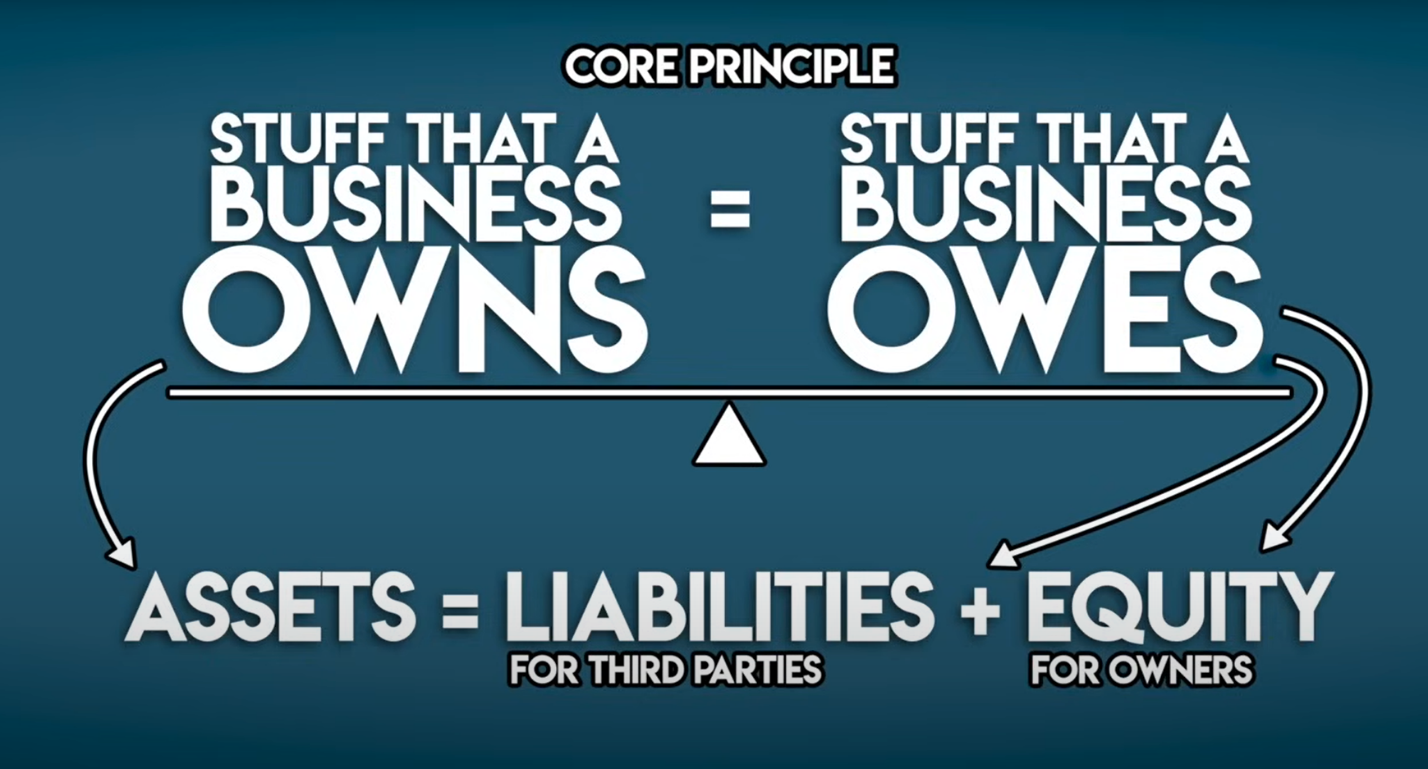
\includegraphics[width=1\textwidth,height=1\textheight,keepaspectratio]{equation.png}
    \caption[short]{\href{https://www.youtube.com/@AccountingStuff}{Accounting Stuff} Principles}
\end{figure}



\section{Accounts (DEA | LER)}
\begingroup
\setlength{\tabcolsep}{75pt}
\renewcommand{\arraystretch}{2}
    \begin{tabular}{ll}
        \toprule
        \key{Debits} & \key{Credits} \\ 
        \midrule
        Dividends & Revenue \\
        Expenses & Equity \\
        Assets & Liabilities \\
        \bottomrule
    \end{tabular}
\endgroup

\section{Debits \& Credits}
\begin{quote}
    They both don’t mean negative or positive. They both counteract each other to make the 
    accounting equation equal. We'll see this more depth in the \hyperref[sec:JournalEntry]{journal entry}. 
\end{quote}

\section{Accrual vs Cash-Basis}
\begin{quote}
    Accrual vs Cash-Basis is the system recording accounts based on \key{different timings}.
    This happens when money leaves and enters the system at different intervals
    like someone paying with their credit-card versus someone paying with cash.
    This allows better organization of accounts within the same period alongside
    following the General Accepted Accounting Principles \key{[GAAP]} or
    International Financial Reporting Standards \key{[IFRS]}. \\\\
    \key{Accrual:} Expenses are recorded when they are incurred \\ 
    Revenue is recognized when it earned, not changed hands. \\

    \key{Cash-Basis: \footnote{Both are regardless on whether money has been exchanged yet}}  
    Expenses are recorded when they are made \\
    Revenue is recorded when it has changed hands.
    
\end{quote}

\section{Double Entry Accounting}

\section{Single Entry Accounting }

\section{§ Accounting Cycle (7 Steps) \protect\footnote{It's generally 8 steps however the General Ledger and General Journal can be combined into one step} }
\begin{enumerate}
    \item Journal Entries
    \item General Ledger \& Journal (2 steps just combined) 
    \item Unadjusted\footnote{ Unadjusted and Ajusted refer to whether it was recorded with cash basis or accrual}  Trial Balance
    \item Adjusting Entries
    \item Ajusted Trial Balance
    \item Financial Statements
    \item Post-Trial Balance
\end{enumerate}

\newpage
\section{Cost Accounting}
Cost Volume Profit Analysis [CVP]
Activity Based Costing (ABC)
Diring and Indirect Costs
Variance Analysis
Overhead and Operating Costs 
LIFO-FIFO
Sarbanes Oxley Act of 2002

\section{Depreciation}
Single Line
Accelerated Decline
Reflecting real world usage 

\section{Ownerships}
\begin{itemize}
    \item Ownership 
    \item Partnership
    \item Corporations \begin{itemize}
        \item Limited Liability Company [LLC]
        \item S-Corp (liability but limited to 100)
        \item C-Corp (unlimited stock quantity)
    \end{itemize}
\end{itemize}

\section{Documents}
Executive Summary
Annual Report
Newletter
10-K 
10-Q 
8-K  
6-K 
S-8 
FORM 3
FORM 4
FORM 5
FORM 144
Proxy Statement
EDGAR